\chapter{Application Development}
\label{ch:application-development}

\section{Overview of the Application}

The application is designed to parse textual input that represents a cause-effect graph, converting it into both a visual and logical format. Upon execution, the system performs two key tasks:

\begin{itemize}
    \item \textbf{Graph Visualization}: The first task is to generate a visualized cause-effect graph from the provided textual input. This allows users to clearly see the logical dependencies between causes (inputs) and effects (outputs), facilitating easy analysis of the business logic. Visual validation of the graph is also possible.
    \item \textbf{Logical Transformation and Decision Table Generation}: In the second phase, the system transforms the cause-effect graph into a logical structure. Through a series of transformation steps, the graph is converted into Boolean logic, and ultimately a decision table is created. This decision table serves as a clear representation of the different logical conditions and their outcomes.
\end{itemize}

All results, including the visual graph, logical transformations, and decision table, are presented in the application's client interface, providing users with an intuitive and comprehensive view of the entire process. The application facilitates the creation of graphical models through a textual interface and displays the transformations leading to the output, which serves as the foundation for generating structured test cases in an optimized manner.

The goal of the application is to simplify and speed up the process of creating cause-effect graphs. Using a textual representation allows for a clearer and more precise definition of the graphs. This approach can effectively represent complex and nested business logic, accommodating various types of rules, causes, and effects.

\section{Application Requirements}

\subsection{Functional Requirements}

Functional requirements describe the core functionalities and capabilities of the application.

\subsubsection{Graph Management}

\begin{compactitem}
	\item The application must allow users to create, edit cause-effect graphs in the live environment.
	\item Users can define variables and rules for the graphs using the custom graph language.
	\item The system must support logical transformations of graphs, including simplification and DNF generation.
	\item The system must offer visualization options for the created graphs.
\end{compactitem}

\subsubsection{Logical Transformation}

\begin{compactitem}
	\item The application must accurately parse logical definitions and simplify them while preserving their original meaning.
	\item Each transformation step should be recorded and made accessible for review.
	\item The final transformation step must result in the Disjunctive Normal Form (DNF) of the logical definitions. Any definition already in DNF should remain unchanged.
\end{compactitem}

\subsubsection{Decision Table Generation}

\begin{compactitem}
	\item The application must generate a decision table based on the defined graphs.
	\item Each rule in the decision table must correspond to logical transformations of the graph.
\end{compactitem}

\subsubsection{Export Functionality}

\begin{compactitem}
	\item The application must support exporting the decision table in General Predicate Testing (GPT) format.
	\item Users can copy the GPT result directly or use a "Copy to Clipboard" button.
\end{compactitem}

\subsection{Non-Functional Requirements}

Non-functional requirements define the quality and performance criteria for the application:

\subsubsection{Performance}

The system should process and render graphs with up to 100 nodes without significant delays (<1 second for transformations). API response times must remain under \emph{500ms} for typical requests.

\subsubsection{Scalability}

The application should be able to handle simultaneous requests from at least \emph{50} users without performance degradation.

\subsubsection{Usability}

The interface must be intuitive, with clear navigation between tabs and pages. Error messages and warnings must be user-friendly and provide actionable guidance.

\subsubsection{Security}

No authentication is required, but the system should prevent unauthorized modifications to predefined graphs or server configurations.

\subsubsection{Compatibility}

The application must be compatible with modern web browsers, including Chrome, Firefox, and Edge.

\subsubsection{Maintainability}

Code should follow clean coding standards with modular and documented components. APIs and Front-end code must be easy to extend to add new features.

\subsubsection{Reliability}

The application should recover gracefully from errors without crashing.

\subsubsection{Portability}

The application must be containerized to ensure seamless deployment in different environments using Docker.

\section{Technical Overview}

The application is built with a focus on efficiently parsing textual inputs, generating cause-effect graphs, and transforming them into logical structures and decision tables. Below is a detailed technical overview of the key components and technologies used in the development process.

\subsection{Technical Stack}

The application is built using a combination of modern technologies, ensuring scalability, maintainability, and ease of development. Below is the breakdown of the technical stack used across various layers of the application.

For detailed information about the codebase, refer to the relevant section in the appendix \ref{sec:dev-env}.

\subsubsection{Front-End (User Interface)}

The first layer, which is directly accessible to end-users, is the user interface or \emph{front-end}. In implementing this, I looked for a modern solution that could meet the application's requirements, providing flexibility and supporting rapid development in a well-structured, maintainable way.

Ultimately, I decided to go with \textbf{ReactJS} \cite{reactjs}, a popular \emph{JavaScript} based library, to build the web-based client application. \textbf{ReactJS} is a widely adopted library for developing user interfaces, particularly in single-page applications where data dynamically changes without requiring a full page reload.

But why \textbf{ReactJS}? \textbf{ReactJS} provides a component-based architecture that is highly modular and reusable, making it an excellent choice for building the dynamic and interactive elements of this application. \textbf{ReactJS} allows us to efficiently manage and update the user interface as users input data and the application generates and visualizes cause-effect graphs.

\textbf{ReactJS}'s strength is in its ability to create highly dynamic, performant, and modular user interfaces. For an application like this, which involves continuous interaction and visualization of cause-effect graphs, React is an excellent choice due to its component-based architecture and efficient handling of frequent updates. However, it does have a learning curve and often requires integrating third-party libraries for advanced features. Despite these challenges, its advantages make it a solid choice for building front-end applications.

\textbf{ReactJS} is a lightweight library on its own, so for more complex and structured solutions, additional tools and libraries are often required. For this project, several other libraries were essential to enhance functionality and streamline development. To align with modern styling principles, I integrated \textbf{Material-UI}, a design library that follows Google's Material Design guidelines, providing a clean and consistent user interface. Additionally, I used \textbf{SCSS} for styling, which offers a modular and maintainable approach to \textbf{CSS}, allowing for better organization and scalability as the application grows.

It's worth highlighting two key libraries that significantly contributed to the functionality of the editor and graph. For the editor, I utilized the Microsoft's \textbf{Monaco Editor}, a modern, lightweight, and highly configurable web-based code editor. This tool enhances user experience by providing helpful hints for structuring graphs. For visualizing the graphs, I integrated the \textbf{Dagre} library, which enables efficient graph rendering, arrangement and visualization.

\subsubsection{Back-End}

The next layer handles the business logic and provides functionality to the clients. For the back-end, I employed \textbf{Ktor}, a \textbf{Kotlin}-based framework designed for building asynchronous servers and web applications. \textbf{Ktor} is known for its flexibility and scalability, allowing developers to create robust \emph{API}s with minimal configuration. Its lightweight architecture makes it particularly well-suited for microservices and cloud-native applications. Additionally, \textbf{Ktor}'s seamless integration with \textbf{Kotlin}'s features, such as coroutines, enhances performance and responsiveness in handling concurrent requests. Overall, \textbf{Ktor} provides an efficient foundation for the back-end of the application, enabling smooth communication between the server and client.

The server's responsibilities include providing initialization data for the client, managing user requests, and executing graph scripts. \textbf{Kotlin} supports its own \emph{Domain-Specific Language} (DSL) implementation, which I utilized in the future development of the application. This \emph{DSL} serves as the backbone of the graphing language, allowing for more expressive and concise syntax when defining cause-effect relationships. By leveraging \textbf{Kotlin}'s \emph{DSL} capabilities, I was able to create a more intuitive interface for users to interact with the graphing functionality, enhancing the overall development experience and usability of the application.

For communication, the server is designed to respond via a \textbf{RESTful API} as well as through \textbf{WebSockets}. The \emph{RESTful API} facilitates standard \textbf{HTTP} requests, enabling seamless interactions between the client and server for data retrieval and manipulation. This allows clients to make synchronous calls for initialization data and other resources.

In addition, the \emph{WebSocket} implementation provides a persistent connection, enabling real-time communication between the client and server. This is primarily used to provide real-time support for the editor.

Currently, the application does not store any data, so there is no need for a connection to a database or any other external storage. Thus, the persistence layer is absent.

\subsubsection{Version Control and CI/CD}

I used \textbf{Git} as the version control system during the development process and \textbf{Microsoft Azure} as the remote server for version control. To enhance searchability, I linked an \textbf{Azure Board} to the repository and created various tasks. Each task's unique identifier is included in the \textbf{Git} commit messages, allowing the server to automatically associate them with the corresponding tasks. Additionally, I used feature branches for implementation and applied Pull Requests for these branches when it was ready to be merged into the main branch. Each request also identifies the connected tasks based on the commit messages.

I also leveraged the \textbf{Microsoft Azure Pipeline} feature to automate the deployment process. These pipelines are automation scripts that, with proper configuration, can automatically generate artifacts from pushed states. I created two pipelines for this project to help validate the correctness of the committed states and automatically generate distribution artifacts.

\begin{itemize}
	\item The first pipeline is dedicated to generating assembled documentation from \textbf{LaTeX}-formatted sources. This pipeline produces a PDF document as an artifact.
	\item The second pipeline focuses on building and packaging the application. It compiles the back-end using \textbf{Gradle} and the front-end using \textbf{Yarn} package manager. Once the build processes are complete, this pipeline packages the compiled front-end code into the back-end package and designates it as an artifact. Additionally, the compiled and built results are packaged into a \textbf{Docker} image with a pre-installed environment and published to the \textbf{Docker Hub} platform. This facilitates deployment in future steps.
\end{itemize}

\subsection{Deployment}

For deployment, I am utilizing \textbf{Docker} with a \emph{Linux-based} environment. \textbf{Docker} enables the application to be packaged and distributed in a way that ensures it can run independently of the underlying platform. This containerization simplifies the deployment process, allowing the application to maintain consistent behavior across various environments.

Why \textbf{Docker}? \textbf{Docker} is an open-source platform that automates the deployment, scaling, and management of applications within lightweight, portable containers. Each container encapsulates an application along with its dependencies, ensuring that it runs consistently across different computing environments, whether in development, testing, or production. \textbf{Docker} streamlines the application development lifecycle by allowing developers to package their applications in a standardized unit, facilitating easier deployment and scaling while minimizing compatibility issues.

The generated \textbf{Docker} images can be used to create containers that are ready for execution. Additionally, these containers assist in scaling performance and availability while preventing overload. With the aid of a \emph{load balancer} and \textbf{Kubernetes}, we can automatically increase the number of containers as needed.

The \textbf{Back-end} operates on port \emph{8080} within the \textbf{Docker} container. It is inaccessible from outside unless an external environment binds an external port to it. Docker facilitates this connection by linking the internal and external ports, creating a bridge between them.

For detailed instructions, refer to the deployment guidelines provided in the appendix \ref{sec:deployment-instructions}.

\subsection{Deployment Requirements}

This section outlines the prerequisites and dependencies necessary for deploying and running the application, including both software and hardware requirements.

\subsubsection{Hardware Requirements}

\begin{compactitem}
	\item \textbf{Processor}: Dual-core CPU or higher.
	\item \textbf{Memory}: Minimum 4 GB RAM
	\item \textbf{Storage}: At least 1 GB of free space for application files and logs.
	\item \textbf{Network}: Internet connection for accessing external APIs or updates.
\end{compactitem}

\subsubsection{Software Requirements}

\begin{compactitem}
	\item \textbf{Operating System}: Windows 10 or later or Linux (Ubuntu 20.04 or equivalent recommended)
	\item \textbf{Memory}: Version 20.10 or later
	\item \textbf{Browser}: Latest versions of Chrome, Firefox, or Edge
\end{compactitem}

Meeting these requirements ensures a smooth setup and operation of the application for both development and end-user usage.

\subsection{Application Architecture}

The architecture of the application is based on a straightforward two-layered model. As the name suggests, the application is divided into two layers: the Front-End and the Back-End. Further details on figure \ref{fig:app-arch}. 

\begin{figure}[H]
	\centering
	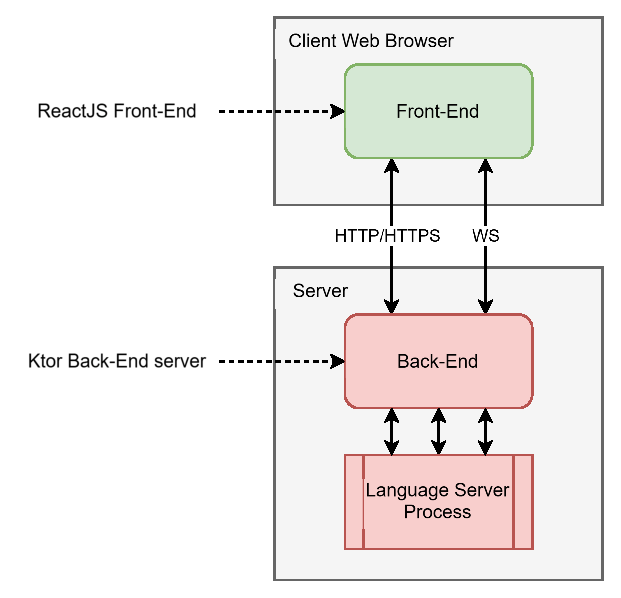
\includegraphics[width=0.5\textwidth,height=200px]{AppArch}
	\caption{Application Architecture}
	\label{fig:app-arch}
\end{figure}

\begin{compactitem}
    \item \textbf{Front-End layer}: This layer is responsible for the user interface and user experience. It handles the presentation of data and interactions with the users, providing a seamless and intuitive interface for creating and managing cause-effect graphs. It is highlighted in green in Figure \ref{fig:app-arch} and operates within the client's web browser.
    \item \textbf{Back-End layer}: This layer manages the application's business logic, data processing, and communication with the front-end. It handles requests from the client, processes them, and sends back the appropriate responses. It is highlighted in red in Figure \ref{fig:app-arch} and operates on a remote server.
\end{compactitem}

The communication between the two layers is bidirectional and can occur via either \emph{HTTP/HTTPS} or \emph{WebSocket} (WS) protocols. 

In the Figure \ref{fig:app-arch}, you can see that the server manages communication with multiple child processes that provide the functionalities of the \textbf{Kotlin Language Server}. Further details about the language server in the section \ref{sec:kotlin-language-server}.

\section{Implementation Details}

Upon accessing the server's address, the user is directed to the web front-end of the application via the index route. From this interface, the user can define a graph through the editor. Once the graph definition is completed and the execution is initiated, the source code is sent to the server for parsing and transformation. The server processes the input and returns the corresponding results, which are then displayed on the client interface.

For a more detailed description of the user interface and its features, see the next \ref{sec:ui} section.

\subsection{Parsing Graph Code}

The first step in the process is parsing the graph code. Once the source code arrives at the server, it is passed to the \textbf{Kotlin Script} parser engine. This engine parses the code and converts it into a \textbf{Kotlin} data model. The data model encapsulates the structure of the graph, including its nodes and relationships. After transforming the textual input, it evolves into this structured model, which can be utilized in subsequent processes.

The \textbf{Kotlin Script} engine can parse \textbf{Kotlin} code in a runtime environment and return the result. This is possible because the graph language is, in fact, a \textbf{Kotlin Script}. By leveraging \textbf{Kotlin}'s \textbf{DSL} (Domain-Specific Language) structure, the language model was developed. The graph language itself consists of a series of \textbf{Kotlin} methods nested within each other, enabling flexible and dynamic representation of the cause-effect graph through executable \textbf{Kotlin} code.

Many \textbf{Kotlin} features enable the created language to be compact and easy to use. Features like extension functions, lambda expressions, and type inference make the syntax more concise, while \textbf{Kotlin}'s strong typing system ensures robustness. These language constructs simplify both the definition and manipulation of the cause-effect graph, allowing for more readable and maintainable code.

\lstset{caption={An example of the graph DSL implementation utilizing Kotlin features.}, label=src:dsl-kotlin}
\begin{lstlisting}[language={Kotlin}]
fun RuleBuilder.cause(
	displayName: String,
	initializer: CauseNodeBuilder.() -> LogicalExpression,
): Node.Cause {
    return CauseNodeBuilder(displayName, variableProvider)
		.apply { expression = initializer() }
		.validateAndBuild()
		.also { cause = it }
}
\end{lstlisting}

In the source code \ref{src:dsl-kotlin}, the function is an extension method of the \texttt{RuleBuilder} class and handles the creation of causes within the context. The method initializes a \texttt{CauseNodeBuilder} with the provided value and applies the external initializer. After initialization, the builder validates its state, and if it is valid, it creates a \texttt{Node.Cause} instance and saves it into the \texttt{RuleBuilder} context. \texttt{Node.Cause} refers to the \texttt{Cause} class, which is an inner class of the \texttt{Node} class.

The source code \ref{src:dsl-kotlin-call} provides an example of calling the code example \ref{src:dsl-kotlin}. When calling the \texttt{cause} function, the \texttt{rule} parent is required because its context is the \texttt{RuleBuilder}. For the \texttt{rule}, the \texttt{GraphBuilder} context is necessary, which is why the \texttt{graph} clause is also included. The details of the language can be found in the section \ref{sec:graph-lang-details}.

\lstset{caption={Invoking the graph DSL example source.}, label=src:dsl-kotlin-call}
\begin{lstlisting}[language={Kotlin}]
graph {
	variables {
		int("a")
	}
	rule {
		cause("C1") { variable("a") eq 1000 }
	}
}
\end{lstlisting}

\subsubsection{Graph Language Details}
\label{sec:graph-lang-details}

\lstset{caption={Definition of a basic rule for the graph}, label=src:basic-rule-def}
\begin{lstlisting}[language={Kotlin}]
import eu.karcags.ceg.graphmodel.dsl.*

graph {
	variables {
		float("budget", 0.01f) // Float variable with name `budget`
	}
	rule {
		cause("C1") { variable("budget") gt 0f }
		effect { "The budget is positive" }
	}
}
\end{lstlisting}

In the code example \ref{src:basic-rule-def}, we see a basic rule definition. After importing the necessary packages, the definition begins with the \texttt{graph} clause, which serves as the root of the language. Everything within the \texttt{graph} block must consist of either rules, variables or meta-cause data.

In \ref{src:basic-rule-def} example, only a single rule has been defined using the \texttt{rule} clause. Each rule must contain at least one cause and one effect, which are created using the \texttt{cause} and \texttt{effect} clauses respectively.

The \texttt{effect} clause contains a string value that represents the effect's description (\emph{The budget is positive}). For the \texttt{cause}, we need to provide a predefined identifier, such as \textbf{"C1"} and the content must include an associated logical expression (\emph{budget > 0}).

The \texttt{rule} clause also includes a \texttt{variables} clause, where the \emph{graph}'s variables can be pre-defined. In this case, a \texttt{Float} variable named "\emph{budget}" is defined with a precision of \emph{0.01}. (In \textbf{Kotlin}, float values are marked with the `\emph{f}` character, so the literal value `\emph{1}` as a float would be written as `\emph{1f}`.)

These expressions also adhere to a specific structural definition. Currently, each expression consists of a logical operator connecting two operands, establishing a basic logical relationship between them.

\begin{table}[H]
	\centering
	\begin{tabular}{ | m{0.11\textwidth} | m{0.27\textwidth} | m{0.52\textwidth} | }
		\hline
		\textbf{Key} & \textbf{Name} & \textbf{Description} \\
		\hline \hline
		\texttt{eq} & Equivalence & The operator is used to define equivalence, establishing that both operands must be logically equal to hold \emph{true}. \\
		\hline
		\texttt{neq} & Inverse Equivalence & The operator serves as the inverse of the \texttt{eq} operator, asserting that the expression is \emph{true} when the two operands are not equal. \\
		\hline
		\texttt{lt} & Lower than & The operator establishes a "less than" relationship between two operands. It is primarily used with numerical values. \\
		\hline
        \texttt{lte} & Lower than or equal & The operator represents the "less than or equal to" operator and also allows for equivalence between the operands. \\
		\hline
        \texttt{gt} & Greater than & The operator signifies "greater than" and is primarily used with numeric operands. \\
		\hline
        \texttt{gte} & Greater than or equal & The "greater than or equal to" operator is like \texttt{gt}, but includes the equality condition. \\
		\hline
        \texttt{isIn} & Is in interval & The operator returns true when the left operand is within the range specified by the right interval literal operand. \\
		\hline
		\texttt{isNotIn} & Is not in interval & The operator is the inverse of the \texttt{isIn} operator. It checks whether the value is \textbf{not} within the given interval. \\
		\hline
	\end{tabular}
	\caption{The logical operators in the graph language}
	\label{tab:graph-lang-logical-operators}
\end{table}

For the operators in the table \ref{tab:graph-lang-logical-operators}, we can use either variables or literals as operands. The literals are primarily equivalent to those in the \textbf{Kotlin} language, but in a restricted form. Five types can be used as expression literals: \textbf{Int}, \textbf{Float}, \textbf{Boolean}, \textbf{Int interval}, and \textbf{Float interval}. Through the \textbf{DSL}'s overloaded functions, only these types are allowed. The table \ref{tab:graph-lang-literals} displays these literal types.

\begin{table}[H]
	\centering
	\begin{tabular}{ | m{0.20\textwidth} | m{0.70\textwidth} | }
		\hline
		\textbf{Type} & \textbf{Description} \\
		\hline \hline
		\textbf{Int} & The standard integer type, ranging from -2,147,483,648 to 2,147,483,647.  \\
		\hline
		\textbf{Float} & Floating-point number type. To use this type, we need to append '\emph{f}' to the end of the number. \\
		\hline
		\textbf{Boolean} & A simple two-value type that only contains `true` and `false`. \\
		\hline
		\textbf{Int interval} & The int range includes all integer values between two given numbers. To define it, we use the `..` operator, for example, \texttt{1..100}, which creates a closed interval. Additionally, an open-ended interval can be defined using the `..<` operator, such as \texttt{1..<100}. \\
		\hline
		\textbf{Float interval} & The float range includes floating values between two given numbers. To define it, we use the `..` operator, for example, \texttt{1f..100f}, which creates a closed interval. Additionally, an open-ended interval can be defined using the `..<` operator, such as \texttt{1f..<100f}. \\
		\hline
	\end{tabular}
	\caption{Allowed literal types and their usage in the graph language}
	\label{tab:graph-lang-literals}
\end{table}

Variables can also be used as operands. These operands represent dynamic (unknown) data in the logical definitions. They can be included using the \texttt{variable} clause, where you simply add the variable's name to the expression. Only pre-defined variables can be referenced within the expressions.

To pre-define variables, you need to fill in the \texttt{variables} clause under the \texttt{graph} clause. There are three types of variables: \textbf{Int}, \textbf{Float}, and \textbf{Boolean}. You can define them using the \texttt{int}, \texttt{float}, and \texttt{boolean} clauses, respectively.

For the \textbf{Int} type, there is no need to define precision, as it is set to \texttt{1} by default. However, for the \textbf{Float} type, specifying precision may be necessary. There is an overloaded \texttt{float} clause where the precision can be defined as the second parameter, following the variable name. The default precision is \texttt{0.1}.

However, the logical expression does not control the operands, as the graph language imposes a key restriction. Each expression must be a \emph{logical} one, where the first operand is a \emph{variable}, and the second is either a \emph{literal} or an \emph{expression} that can be simplified to a literal.

In the \ref{src:basic-rule-def} example, the expression for the \textbf{C1} cause represents a straightforward equivalence between the \emph{literal} 1000 and the \emph{variable} \textbf{a}.

In the following example \ref{src:complex-rule-def}, we see more complex rule definitions. By utilizing the repeated \texttt{rule} clause, additional rule definitions can be incorporated within the graph.

\lstset{caption={Definition of a complex rules for the graph}, label=src:complex-rule-def}
\begin{lstlisting}[language={Kotlin}]
import eu.karcags.ceg.graphmodel.dsl.*

graph {
	variables {
		boolean("validUsername")
		boolean("validPassword")
		boolean("validAccessToken")
		int("loginAttempt")
	}
	cause("CATTEMPT") { variable("loginAttempt") gt 3 }
	rule {
		causeById("CATTEMPT")
		effect { "Block further login possibilities" }
	}
	rule {
		and {
			or {
				cause("C21") { variable("validAccessToken") eq true }
				and {
					cause("C22") { variable("validUsername") eq true }
					cause("C23") { variable("validPassword") eq true }
				}
			}
			not { causeById("CATTEMPT") }
		}
		effect { "Access is granted" }
	}
}
\end{lstlisting}

A new cause type has been introduced in the new graph definition. Unlike regular causes, which are defined within a rule, these are defined at the graph level, making them not directly connected to any specific rule by default. These are referred to as meta-causes. This feature allows users to reuse existing cause definitions across different rules, enhancing modularity and efficiency. Aside from these differences, the \texttt{cause} clause functions in the same way as it does at the rule level.

In the first and second rule definitions, there are examples of the cause reusing. By utilizing the \texttt{causeById} clause along with a unique name, the previously defined cause can be referenced. With this solution, all causes can be reused, but each cause can only be defined once in a graph.

Certainly, these basic causes alone are insufficient to construct complex business logic within the graph. Therefore, it's possible to encapsulate the \texttt{cause} clauses within logical clauses such as \texttt{or}, \texttt{and}, or \texttt{not}. These operators merely wrap the defined causes, allowing for more intricate relationships and logic.

In the \texttt{not} clause, only a single child can be encapsulated, whereas the \texttt{or} and \texttt{and} clauses require at least two children. This distinction allows for different logical structures and complexity within the graph.

These logical clauses can be nested independently within each other; however, at the end of each logical tree, a cause definition must be present. This ensures that every logical expression ultimately relates back to specific causes.

The first rule references the pre-defined meta-cause for blocking further login attempts, while the second rule defines a complex structure for granting access. In this example, access is granted if the login attempt limit has not been reached and a valid access token is provided, or if a valid username-password pair is submitted.

\subsection{Transform Into Visual Graph}

Once the source code is parsed, the resulting graph model serves as the foundation for subsequent processes and transformations. One of these processes involves generating a visual representation of the graph for Front-End visualization.

The process is straightforward. From the graph model, all visual nodes are identified. The node discovery is an uncomplicated procedure. First, the algorithm locates all effects in the model and converts them into graph nodes. Next, all causes are similarly transformed into graph nodes. The graph visualizes the logical relationships between these nodes, thus all logical connections among the cause nodes are also represented as graph nodes.

Alongside node detection, we also need to gather the edges for the graph. These edges represent the one-way arrow connections between the nodes. If a rule contains only one cause definition, the graph visualization for that rule will consist of two nodes connected by an arrow from the cause to the effect. However, if the cause involves a complex nested relation, the logical nodes created will be traversed as part of the rule's graph flow.

Let's examine an example. The source code \ref{src:complex-rule-def} is visualized as shown in the figure \ref{fig:complex-graph-def}.

\begin{figure}[H]
	\centering
	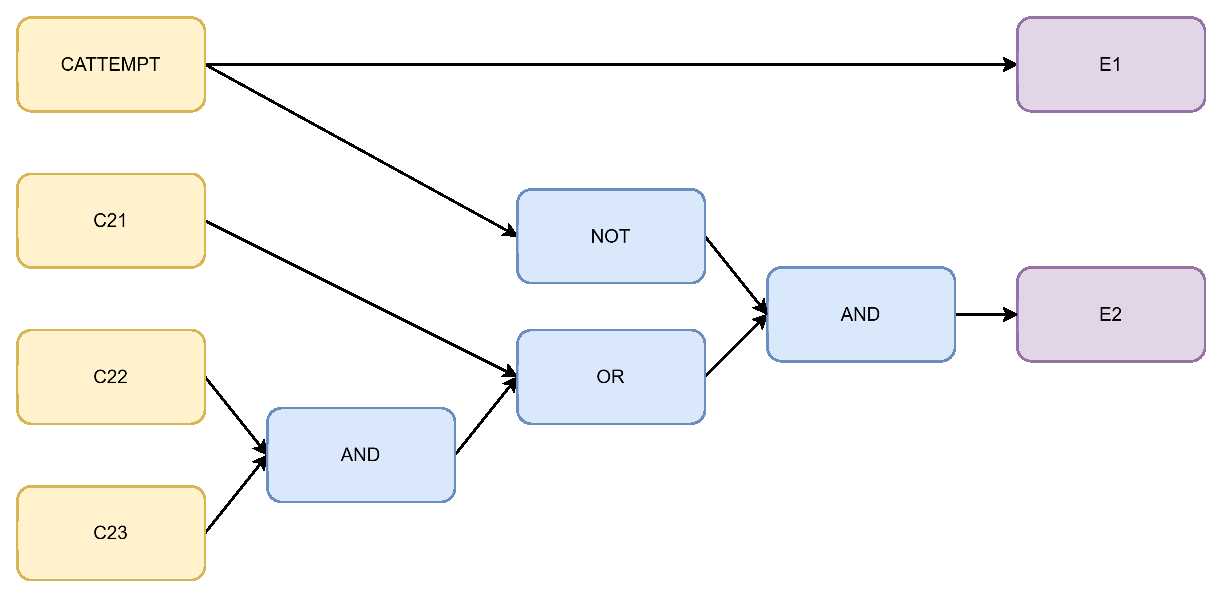
\includegraphics[width=0.9\textwidth,height=210px]{ComplexGraphDef}
	\caption{Visual graph representation of \ref{src:complex-rule-def} graph}
	\label{fig:complex-graph-def}
\end{figure}

The transformation result will yield a collection of independent nodes along with a set of edges, which include references for both the starting and ending points. This output is easily interpretable by the \textbf{Front-end}, enabling it to render the graph accordingly.

\subsection{Transfrom Into Logical Formulas}

The transformation involves a straightforward translation between the graph model and logical formulas, along with various logical formula refiners that perform modifications, optimizations, and simplifications.

\subsubsection{Translate Graph Model into Logical Formulas}

In the first step each rule in the graph is translated into logical definition pairs. The first element of the pair represents the destination effect, serving as a symbolic entry that corresponds to the second element, which is a combined logical definition. This definition is constructed from the rule's \texttt{cause} clauses or the wrapping logical operator clauses. The transformation process is straightforward, with each clause representing its own logical definition. The \texttt{and} clause will be represented as an \textbf{AND} object, while the \texttt{cause} clause will simply become a standalone logical node.

Let's examine the first step in the previously mentioned example \ref{src:basic-rule-def}. The translation process for this single-rule graph is quite straightforward.

\begin{compactitem}
	\item $ E1 = C1 $
\end{compactitem}

The representation is straightforward, with an equivalence between \textbf{E1} and \textbf{C1}. However, all node metadata is stored in the underlying data model. To see a more complex result, let's examine the \ref{src:complex-rule-def} example.

\begin{compactitem}
	\item $ E1 = CATTEMPT $
	\item $ E2 = (C21 \lor (C22 \land C23)) \land \lnot CATTEMPT $
\end{compactitem}

In this case, there are two rules. The first rule is a simple equivalence between a cause and an effect, but the second is more complex, involving nested structures with logical operators like \textbf{AND}, \textbf{OR}, and \textbf{NOT}. These operators combine multiple causes, making the resulting logical expressions more intricate.

\subsubsection{Refining of Logical Formulas}

The straightforward translation of the rules into logical formulas is insufficient for subsequent steps, such as decision table creation or test generation. Therefore, we need to further refine and modify these formulas to ensure they are usable in those processes. This includes simplification, normalization, and possibly restructuring the logic for better test coverage and decision-making accuracy.

In the application, the logical formula system undergoes a refiner pipeline, where each step in the pipeline modifies some aspect of the formula structure. These refiners apply transformations such as simplifications, optimizations, and logical normalizations. The output from one refiner serves as the input to the next, ensuring that by the end of the pipeline, the logical formula system is well-structured, optimized, and ready.

The list of the refiners:

\begin{itemize}
	\item \textbf{Negation Inward Mover}: The first element of the pipeline is responsible for pushing all negations inward within the logical definition. Using \textbf{De Morgan's law}, any negation is moved deeper into the structure, applying directly to the individual nodes. This process ensures that negations only appear at the operand level. Additionally, any duplicate or unnecessary negations are eliminated during this step, simplifying the overall structure of the formula.
	\item \textbf{Binary Collapser}: In this step, the system collapses identical binary operators, such as \textbf{AND} and \textbf{OR}. If a binary operator has neighboring operators of the same type, the system merges them to simplify the definition and eliminate unnecessary redundancies.
	\item \textbf{Opposition Eliminator}: The next step removes all tautologies from the \textbf{OR} definitions. If an \textbf{OR} operation contains both a logical definition and its negation, the system eliminates the redundant items from further processing.
	\item \textbf{DNF}: The last element of the pipeline focuses on converting the logical formula into \textbf{DNF}. The algorithm processes all complex or convertible logical definitions, breaking them down into a full \textbf{DNF}, where the formula is expressed as a disjunction of conjunctions. Any simple logical definitions that are already in their simplest form are left unchanged, ensuring efficiency while maintaining the integrity of the logical structure.
\end{itemize}

\subsection{Construct Decision Table}

After passing through the pipeline of refinement steps, the logical formulas are fully optimized and ready for the conversion. This conversion process transforms the refined logical expressions into a structured table that clearly defines the relationships between various causes and their corresponding effects.

The optimized DNF rules are now ready to be translated into a Decision Table. The process involves individually constructing each logical definition into at least one column. For simple definitions, such as single-node conditions or basic \textbf{AND} operations, each is translated directly into a single column. This is because they can be expanded into a disjunction containing only one item.

After the DNF transformation, more complex items (those that are disjunctions of conjunctions) must be represented as multiple columns in the decision table. Each conjunction within the disjunction becomes a separate column, and all columns for a given rule will share the same effect.

For example, let's look at the second rule from the previous example and how it would appear in table format:

\begin{table}[H]
	\centering
	\begin{tabular}{ | m{0.17\textwidth} | m{0.12\textwidth} | m{0.12\textwidth} | m{0.12\textwidth} | m{0.12\textwidth} | }
		\hline
		\textbf{Nodes} & \textbf{Rule 1} & \textbf{Rule 2} & \textbf{Rule 3} & \textbf{Rule 4} \\
		\hline \hline
		\emph{C21} & - & 1 & - & 1 \\
		\hline
		\emph{C22} & - & 0 & 1 & - \\
		\hline
		\emph{C23} & - & 1 & 1 & 0 \\
		\hline
        \emph{CATTEMPT} & 1 & 0 & 0 & 0 \\
		\hline \hline
        \emph{E1} & 1 &   &   &   \\
		\hline
		\emph{E2} &   & 1 & 1 & 1 \\
		\hline
	\end{tabular}
	\caption{The decision table of the \ref{src:complex-rule-def} graph definition}
	\label{tab:complex-graph-decision-table}
\end{table}

For the first rule, only a single column is needed in the decision table, as their logical structure is simple. However, the second graph rule requires three columns because its simplified DNF form is a disjunction of three elements. Each element can cause the activation of the corresponding effect.

\subsection{Export}

The final step in the process is generating the export. This is a crucial phase, as the application's outputs can be utilized by other tools to create test cases.

At present, the system generates a single export. Based on the constructed decision table, a text file is created in the General Predicate Testing (GPT) format, serving as input for a test generator.

\subsubsection{GPT (General Predicate Testing)}

\lstset{caption={GPT result of the \ref{src:complex-rule-def} graph definition}, label=src:gpt-export-complex-rule-def}
\begin{lstlisting}
loginAttempt(int);validAccessToken(bool);validUsername(bool);validPassword(bool)
>3;*;*;*
<=3;true;false;true
<=3;*;true;true
<=3;true;*;false
\end{lstlisting}

A GPT result adheres to a straightforward structure. The output is derived from the constructed decision table, with most of its elements represented in an alternate format.

The first row of the result lists all the variables used, along with their types and precision (for float variables). The subsequent rows correspond to the columns of the decision table. Each variable used is gathered from the cause definitions, and the logical expressions are included. All logical operators can be converted into this structured format.

As shown in the result \ref{src:gpt-export-complex-rule-def}, four variables have been defined, and four rules have been converted. Each definition aligns with the variable types: for boolean variables, \texttt{true} and \texttt{false} are used, while numerical variables include other operators. When a variable is not used in a specific rule, it is indicated with a `\emph{*}`. The table \ref{tab:gpt-logical-conversion-table} illustrates the conversion of expressions.

\begin{table}[H]
	\centering
	\begin{tabular}{ | m{0.40\textwidth} | m{0.40\textwidth} | }
		\hline
		\textbf{Operator} & \textbf{GPT result} \\
		\hline \hline
		\texttt{"a" eq 12} & =12 \\
		\hline
		\texttt{"a" neq 12} & !=12 \\
		\hline
		\texttt{"a" lt 12} & <12 \\
		\hline
        \texttt{"a" lte 12} & <=12 \\
		\hline
		\texttt{"a" gt 12} & >12 \\
		\hline
		\texttt{"a" gte 12} & >=12 \\
		\hline
		\texttt{"a" isIn 1..12} & [1,12] \\
		\hline
		\texttt{"a" isIn 1..<12} & [1,12) \\
		\hline
	\end{tabular}
	\caption{GPT logical conversion table}
	\label{tab:gpt-logical-conversion-table}
\end{table}

\subsection{Technical Details}

\subsubsection{Authentication}

The application does not require authentication to access its features. All functions are available anyone. It makes the application more dynamic and user-friendly, while being less restrictive.

\subsubsection{Authorization}

The application has no various restriction levels and due to its minimal functionality, all features are accessible to everyone. Since there are no users or data storage involved, there are no restricted elements.

\subsubsection{Front-end endpoints}

The application is primarily a single-page application, but it consists of three different pages. The index route (\texttt{/}) displays the main functionality in a tabbed view, while the other two pages are simple visualization pages with no user interaction.

The \texttt{/about} page provides information about the application and its creator, while the \texttt{/docs} page contains documentation for the graph language.

\subsubsection{Back-end endpoints}

The \textbf{Back-end} offers additional endpoints, primarily focused on graph functionality, with others related to the editor. The table \ref{tab:backend-endpoints} presents all the available and used endpoints.

\begin{table}[H]
	\centering
	\begin{tabular}{ | m{0.3\textwidth} | m{0.12\textwidth} | m{0.48\textwidth} | }
		\hline
		\textbf{Path} & \textbf{Method} & \textbf{Description} \\
		\hline \hline
		\texttt{/graph/initial} & \texttt{GET} & Returns the initial content of the editor. \\
		\hline
		\texttt{/graph/parse/all} & \texttt{POST} & Parses the input source code and returns all the corresponding transformations and exports. \\
		\hline
		\texttt{/graph/examples} & \texttt{GET} & Returns the keys of all the pre-defined example graphs. \\
		\hline
		\texttt{/graph/examples/{key}} & \texttt{GET} & Returns all transformations and exports for the example graph associated with the given key. \\
		\hline
	\end{tabular}
	\caption{Available \textbf{Back-end} endpoints}
	\label{tab:backend-endpoints}
\end{table}

\section{User Interface}
\label{sec:ui}

The user interface of the application is designed to be simple and lightweight. It follows a single-page layout that effectively accommodates the main functionalities. The key features are organized in a tabbed format, with each feature residing in its own dedicated tab. This structure ensures that users can easily navigate between different functionalities without unnecessary complexity, enhancing the overall user experience.

\subsection{Editor}

By default, the \textbf{Editor} tab is selected, and all other tabs are disabled, as there is no valid graph definition present initially. The editor's initial content includes only an \emph{import} statement and a \emph{graph} clause with \emph{variables} and \emph{rule} blocks, offering a clean and minimalistic environment for users to start defining their cause-effect graphs. This state can be seen in the figure \ref{fig:ui-editor-init}.

\begin{figure}[H]
	\centering
	\includegraphics[width=1\textwidth,height=260px]{UserInterface-Editor-Initial}
	\caption{User Interface - Editor tab - Initial state}
	\label{fig:ui-editor-init}
\end{figure}

Below the editor, there is a message box that displays the results of each execution and other information. It shows either successful execution messages or error responses. For convenience, the messages block can be collapsed and expanded as needed.

Below the messages box is an action row containing three buttons and a warning message. The warning message is displayed only when the most recent execution was invalid or if the current editor state has been modified since the last execution.

On the right side of the action row are two buttons that control the editor. The first is the \textbf{Reset} button, which restores the editor's content to its initial state, discarding any changes. The second is the \textbf{Execute} button, which is initially disabled. When the user modifies the editor's content, the \textbf{Execute} button becomes enabled and ready for use.

When the \textbf{Execute} button is clicked, the client sends the content of the editor to the server for evaluation. If the execution encounters any errors, an error message will be displayed in the mentioned messages box, indicating the unsuccessful execution. In other cases, the system will parse the content and define the graph. Once the conversions are complete, the results will activate the other tabs, allowing users to access the newly generated information.

Located on the left side of the action row, the \textbf{Docs} button opens a dialog when clicked. This dialog appears above all other \emph{UI} elements and provides a brief overview of the language, its commands, and some examples. This can be seen in the figure \ref{fig:ui-editor-docs}.

\begin{figure}[H]
	\centering
	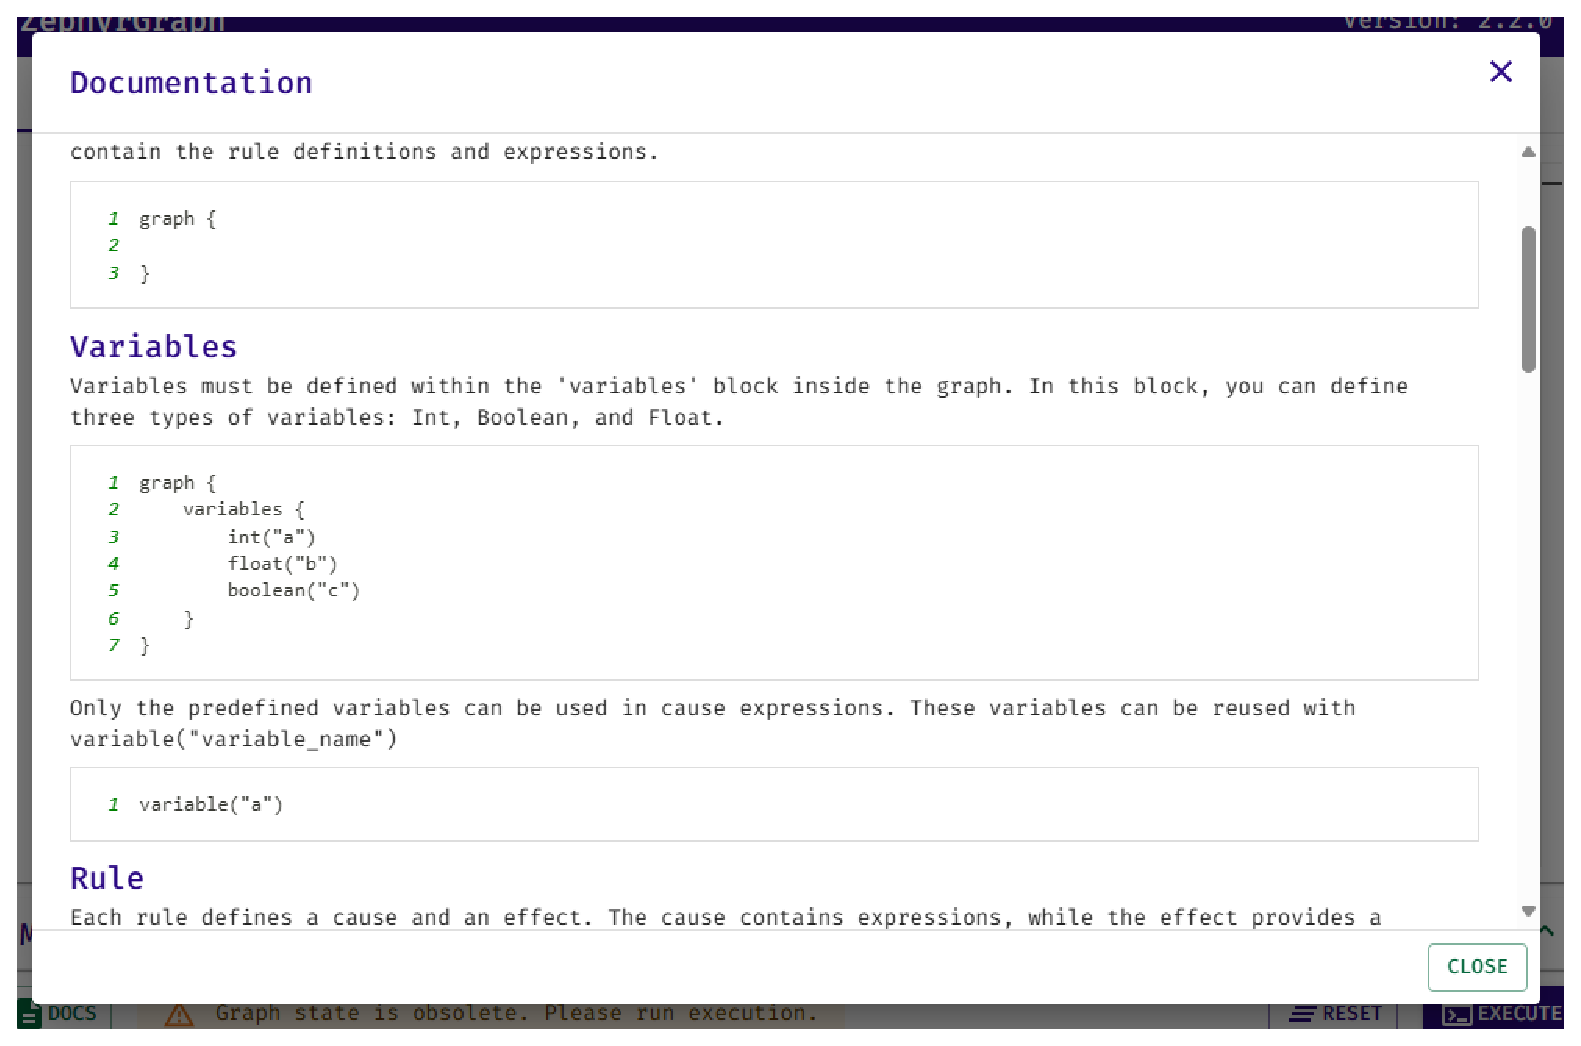
\includegraphics[width=1\textwidth,height=260px]{UserInterface-Editor-Docs}
	\caption{User Interface - Editor tab - Documentation}
	\label{fig:ui-editor-docs}
\end{figure}

The editor assists users by providing color coding and code IntelliSense features, which include helpful snippets. These enhancements improve the user experience by making it easier to write and understand the graph definitions, reducing the likelihood of errors and streamlining the overall editing process.

\begin{figure}[H]
	\centering
	\includegraphics[width=1\textwidth,height=260px]{UserInterface-Editor-Filled}
	\caption{User Interface - Editor tab - With an executed example}
	\label{fig:ui-editor-filled}
\end{figure}

\subsection{Logical Results}

After a successful execution, the tabs that depend on the \textbf{Editor} will become available. The \textbf{Logical Results} tab displays the logical formulas parsed from the graph language, along with the corresponding logical formulas after the transformation steps. Each transformation step is presented for each rule, providing a clear overview of the progression from the initial graph to the final logical representation.

\begin{figure}[H]
	\centering
	\includegraphics[width=1\textwidth,height=260px]{UserInterface-LogicalResults}
	\caption{User Interface - Logical Results tab}
	\label{fig:ui-logical-results}
\end{figure}

As shown in the figure \ref{fig:ui-logical-results}, the steps are in reverse order. The initial state is the last element, and each subsequent step represents the preceding one. The final state appears as the first element. Each step illustrates the constructed logical definition based on the rules. The final state, the DNF, will serve as the basis for the next tab, the Decision Table.

\subsection{Decision Table}

From the final logical results, the system generates a decision table, which is displayed on the third tab. Each rule is converted into one or more columns in the table. Each column collects the causes and their corresponding values necessary to invoke a specific effect, providing a clear and organized representation of the decision-making logic for the further test generation process.

\begin{figure}[H]
	\centering
	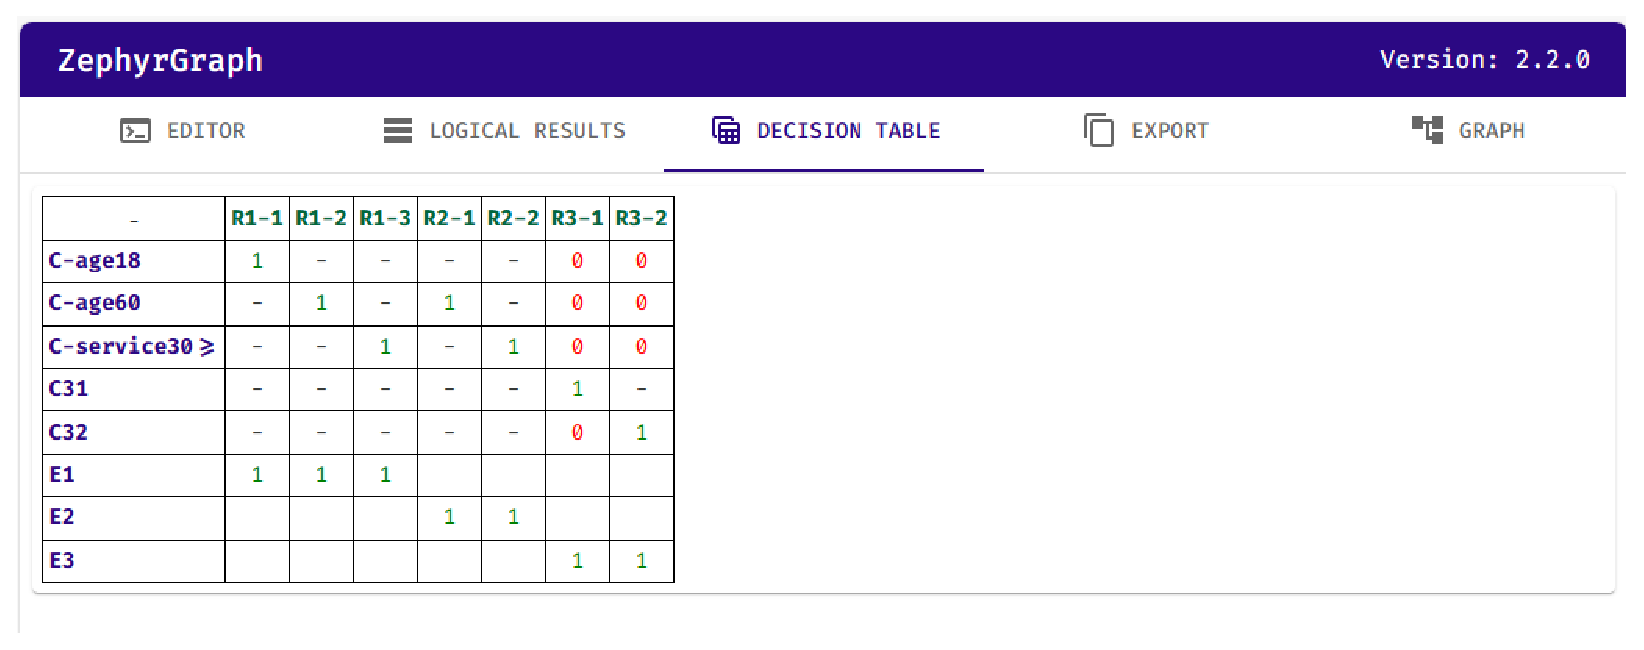
\includegraphics[width=1\textwidth,height=140px]{UserInterface-DecisionTable}
	\caption{User Interface - Decision Table tab}
	\label{fig:ui-decision-table}
\end{figure}

The figure \ref{fig:ui-decision-table} displays the table where \emph{ones (green)} represent \emph{true} values and \emph{zeros (red)} represent \emph{false} values. If a cell is empty or contains a hyphen, it is not part of the new logical definition. Only one effect can be marked in each column, and it cannot be marked as a false value.

\subsection{Export}

The fourth tab contains the available export options. Currently, the only export format is the GPT (General Predicate Testing) structured text result, which is generated from the decision table.

\begin{figure}[H]
	\centering
	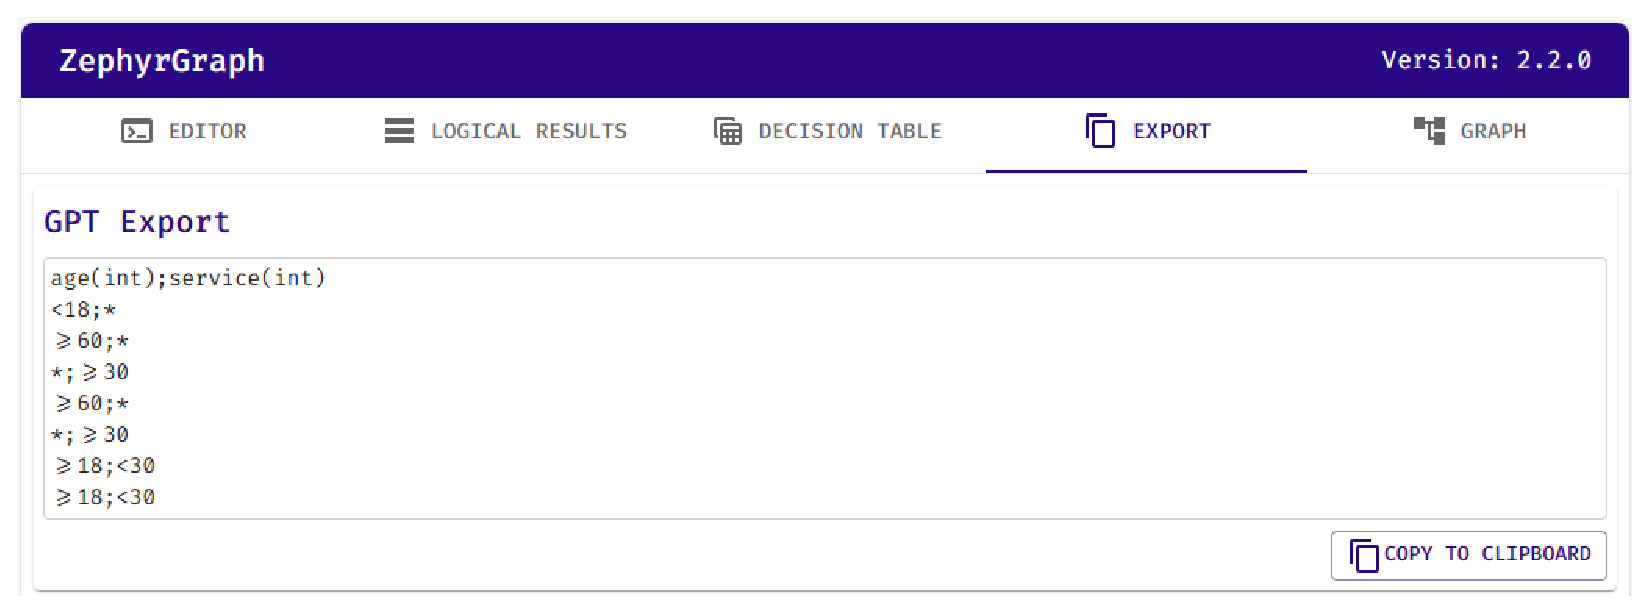
\includegraphics[width=1\textwidth,height=140px]{UserInterface-Export}
	\caption{User Interface - Export tab}
	\label{fig:ui-export}
\end{figure}

The figure \ref{fig:ui-export} displays the output of the current example. You can either select the value to copy and paste it manually, or use the \textbf{Copy to Clipboard} button for a quicker option.

\subsection{Graph}

On the final tab, a visual representation of the defined graph is displayed. Each node, including causes, effects, and logical nodes, is represented in different colors for easy identification. The nodes are connected to one another by directed arrows, which serve as edges, clearly illustrating the relationships and flow between the various components of the graph.

\begin{figure}[H]
	\centering
	\includegraphics[width=1\textwidth,height=260px]{UserInterface-Graph}
	\caption{User Interface - Graph tab}
	\label{fig:ui-graph}
\end{figure}

The figure \ref{fig:ui-graph} shows the graph of the example, with all effects colored in a shade of red, logical nodes in orange, and causes in yellow.

\section{Kotlin Language Server}
\label{sec:kotlin-language-server}

To support client-side editing in the Monaco editor, a \textbf{Kotlin Language Server} connection was implemented. When the client editor initializes, it sends a connection request to the \textbf{Back-End}'s socket interface. This interface is responsible for setting up and managing the connection between the client and the language server, allowing real-time code analysis, syntax highlighting, and other editor features to enhance the user experience.

Upon initialization, the \textbf{Back-End} starts the \textbf{Kotlin Language Server} as a child process. When a message arrives at the \textbf{Back-End}, it processes the message and then forwards it to the language server. Each response from the language server is similarly handled by the \textbf{Back-End} and relayed back to the client via the established \textbf{Socket} connection. This setup ensures smooth communication between the client editor and the language server, allowing for real-time feedback and interaction.

The syntax of the graph language has been integrated into the language server as an external library. This allows the language server to offer reliable assistance during editing, including features like code completion, syntax highlighting, and error detection, enhancing the overall user experience.

\begin{figure}[H]
	\centering
	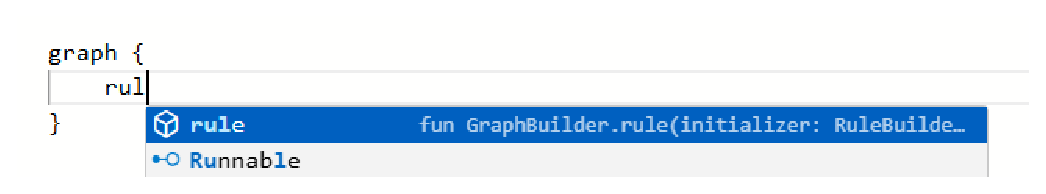
\includegraphics[width=0.8\textwidth,height=60px]{Intellisense}
	\caption{Monaco Editor intellisense for the graph language}
	\label{fig:editor-intellisense}
\end{figure}